%
% $Id: $
%
%
% Compilar a .pdf con LaTeX (pdflatex)
% Es necesario instalar Beamer (paquete latex-beamer en Debian)
%

%
% Gráficos:
% Los gráficos pueden suministrarse en PNG, JPG, TIF, PDF, MPS
% Los EPS deben convertirse a PDF (usar epstopdf)
%

\documentclass{beamer}
\usetheme{JuanLesPins}
%\usebackgroundtemplate{\includegraphics[width=\paperwidth]{format/gsyc-bg.png}}
%\usepackage[spanish]{babel}
\usepackage[latin1]{inputenc}
\usepackage{graphics}
\usepackage{amssymb} % Simbolos matematicos

%\definecolor{libresoftgreen}{RGB}{162,190,43}
%\definecolor{libresoftblue}{RGB}{0,98,143}

%\setbeamercolor{titlelike}{bg=libresoftgreen}

%% Metadatos del PDF.
\hypersetup{
  pdftitle={PTAVI :: Presentación Práctica Final},
  pdfauthor={Gregorio Robles, Jesús M. González Barahona},
  pdfcreator={GSyC, Universidad Rey Juan Carlos},
  pdfproducer=PDFLaTeX,
  pdfsubject={PTAVI :: Presentación Práctica Final},
}
%%

\begin{document}

\title{Presentación de la Práctica Final}
\subtitle{Protocolos para la Transimisión de Audio y Vídeo por Internet}
\institute{grex@gsyc.urjc.es \\
GSyC, Universidad Rey Juan Carlos}
\author{Gregorio Robles}
\date{25 de noviembre de 2019}

\frame{
\maketitle
}


% Si el titulo o el autor se quieren acortar para los pies de página
% se pueden redefinir aquí:
%\title{Titulo corto}
%\author{Autores abreviado}


%% LICENCIA DE REDISTRIBUCION DE LAS TRANSPAS
\frame{
~
\vspace{4cm}

\begin{flushright}
{\tiny
(cc) 2008-19 Gregorio Robles, Jesús M. González Barahona \\
  Some rights reserved. This work licensed under Creative Commons \\
  Attribution-ShareAlike License. To view a copy of full license, see \\
\ \\
  http://creativecommons.org/licenses/by-sa/3.0/ or write to \\
  Creative Commons, 559 Nathan Abbott Way, Stanford, \\
  California 94305, USA. \\

}
\end{flushright}
}

\section{Recordatorio de Evaluación de PTAVI}

\begin{frame}
\frametitle{Evaluación}

\begin{itemize}
  \item Prácticas: hasta 5,5 puntos. \\ Mínimo: Parte básica práctica final.
  \item Teoría: hasta 5 puntos. \\ Mínimo: Superar la evaluación final de teoría.
  \item Al sumar teoría y prácticas, la suma ha de dar un 5 o más.
\begin{itemize}
  \item Entrega práctica final parte básica: 0 puntos
  \item Requisitos avanzados práctica final: hasta 2 puntos
\end{itemize}
\end{itemize}

\end{frame}


\begin{frame}
\frametitle{Práctica final}

\begin{itemize}
  \item Individual
  \item De obligatorio cumplimiento (i.e., sin las prácticas aprobadas, no se aprueba la asignatura)
  \item Realizadas en Python
  \item Temática: servicio SIP
  \item Fecha de entrega: 23.12.2019 a las 12:00 (ofrece la posibilidad de hacer partes opcionales)
  \item Fecha de entrega: 10.1.2020 a las 12:00
  \item Habrá clases específicas de apoyo a la práctica final
  \item Habrá tutorías en el laboratorio (lunes 2.12 a las 9:00, miércoles 3.12 a las 9:00, miércoles 11.1 a las 9:00)
  \item Hay instrucciones (muy) detalladas en el guión
  \item Atención: el guión podría cambiar ligeramente durante los próximos días
\end{itemize}

\end{frame}

%%

\section{Práctica Final}

\begin{frame}
\frametitle{Objetivo Principal}

\begin{center}
  \begin{huge}
    Implementar un servicio SIP sencillo, pero completo.
  \end{huge}
\end{center}

\end{frame}

%%%%%%%%%%%%%%%%%%%%%%%%%%%%%%%%%%%%%%%%%%%%%%%%%%%%%%%%%%%%%%%%%%%%%%%

\begin{frame}
\frametitle{Requisitos mínimos}

\begin{itemize}
\item SIP User Agent (cliente y servidor). Pueden ejecutarse por separado.
\begin{itemize}
  \item Descripción de sesión con SDP
\end{itemize}
\item Servidor Registrar y Proxy SIP (un único servidor real)
\begin{itemize}
  \item Base de datos de usuarios registrados en fichero de texto
  \item \emph{time out}
\end{itemize}
\item Envío RTP (con mp32rtp)
\item En todos los clientes y servidores:
\begin{itemize}
  \item Configuración por defecto almacenada en un archivo XML.
  \item Mensajes de log en fichero de texto.
\end{itemize}

\end{itemize}

\end{frame}


%%%%%%%%%%%%%%%%%%%%%%%%%%%%%%%%%%%%%%%%%%%%%%%%%%%%%%%%%%%%%%%%%%%%%%%

\begin{frame}
\frametitle{Requisitos}

\begin{itemize}
  \item El protocolo SIP se debe seguir estrictamente
  \item Los nombres de los programas vienen especificados
  \item Los parámetros de los programas han de ser los que se indican
  \item El formato de los logs está definido
  \item Algunos mensajes de error vienen definidos
  \item Para el resto de cosas, incluida la implementación, se puede hacer 
como se desee
\end{itemize}


\end{frame}

%%%%%%%%%%%%%%%%%%%%%%%%%%%%%%%%%%%%%%%%%%%%%%%%%%%%%%%%%%%%%%%%%%%%%%%

\begin{frame}
\frametitle{SIP: Session Initiation Protocol}

\begin{itemize}
  \item Métodos: REGISTER, ACK, INVITE, BYE
  \item Códigos de respuesta: 100, 180, 200, 400, 401, 404, 405
  \item El registro es autenticado
  \item Detalles en el documento con instrucciones
\end{itemize}


\end{frame}




%%%%%%%%%%%%%%%%%%%%%%%%%%%%%%%%%%%%%%%%%%%%%%%%%%%%%%%%%%%%%%%%%%%%%%%

\begin{frame}
\frametitle{Servidor Registrar}

\begin{itemize}
  \item Configuración almacenada en XML
  \begin{itemize}
    \item puerto donde estará el servidor escuchando, nombre del servidor, ruta del fichero de \emph{log}, tiempo de \emph{time out} de registro (en segundos), ruta del binario mp32rtp (ver más abajo) y ruta de la canción MP3 a enviar (ver más abajo).
   \end{itemize}
   \item Diccionario y fichero (consistencia). Patrón \emph{singleton}
   \item En caso de caída, leemos del fichero los usuarios registrados
   \item El registro es autenticado
\end{itemize}

\end{frame}

%%%%%%%%%%%%%%%%%%%%%%%%%%%%%%%%%%%%%%%%%%%%%%%%%%%%%%%%%%%%%%%%%%%%%%%

\begin{frame}[fragile]
\frametitle{Mensajes de log}

Ejemplo:

\begin{footnotesize}
\begin{verbatim}
...
20161128152045 Starting...
20161128153012 Sent to 127.0.0.1:5555: REGISTER sip:leonard@bigbang.org:1234 SIP/2.0 [...]
20161128153017 Received from 127.0.0.1:5555: 200 OK [...]
20161128153036 Sent to 127.0.0.1:5555: INVITE penny@girlnextdoor.com [...]
...
20161128160035 Sent to 127.0.0.1:5555: BYE [...]
20161128160035 Received from 127.0.0.1:5555: 200 OK [...]
20161128160112 Finishing.
\end{verbatim}
\end{footnotesize}
\end{frame} 

%%%%%%%%%%%%%%%%%%%%%%%%%%%%%%%%%%%%%%%%%%%%%%%%%%%%%%%%%%%%%%%%%%%%%%%

\begin{frame}[fragile]
\frametitle{SDP: Session Description Protocol}

Ejemplo de cuerpo de mensaje con SDP (ojo, esto sólo es el cuerpo):

\begin{verbatim}
v=0
o=grex@direccion.dom 193.147.71.99
s=misesion
t=0 
m=audio 12345 RTP
\end{verbatim}

\end{frame} 

%%%%%%%%%%%%%%%%%%%%%%%%%%%%%%%%%%%%%%%%%%%%%%%%%%%%%%%%%%%%%%%%%%%%%%%

\begin{frame}[fragile]
\frametitle{Envío RTP}

\begin{itemize}
  \item mp32rtp
  \item Hace falta descargarlo, y darle permisos de ejecución
  \item Ver README para su ejecución: 

\begin{verbatim}
./mp32rtp -i direccionIP -p puerto < cancion.mp3
\end{verbatim}
  \item Instrucciones detalladas en el documento de la práctica final
  \item No hace falta escuchar la canción
\end{itemize}

\end{frame} 

%%%%%%%%%%%%%%%%%%%%%%%%%%%%%%%%%%%%%%%%%%%%%%%%%%%%%%%%%%%%%%%%%%%%%%%

\begin{frame}
\frametitle{Ejemplo de una sesión SIP}

\begin{center}
  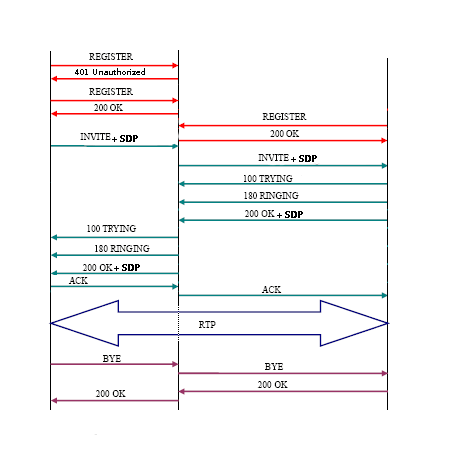
\includegraphics[width=8cm]{figs/complete-sip-session.png}
\end{center}


\end{frame}


%%%%%%%%%%%%%%%%%%%%%%%%%%%%%%%%%%%%%%%%%%%%%%%%%%%%%%%%%%%%%%%%%%%%%%%
%
%\begin{frame}
%\frametitle{Criterios secundarios dde evaluación}
%
%\begin{itemize}
%  \item Legibilidad del código y seguimiento de la guía de estilo de Python
%  \item Comprobación de mensajes SIP y archivos de \emph{log} para que sigan las instrucciones
%  \item Los servidores y clientes se comunican con los 
%\end{itemize}
%
%\end{frame}

%%%%%%%%%%%%%%%%%%%%%%%%%%%%%%%%%%%%%%%%%%%%%%%%%%%%%%%%%%%%%%%%%%%%%%%

\begin{frame}
\frametitle{Requisitos Avanzados}

\begin{itemize}
  \item Para realizarlas, hay que entregar la parte opcional antes de Navidades
  \item Se presentan en un documento aparte, que se publicará en breve
\end{itemize}

\end{frame}

%%%%%%%%%%%%%%%%%%%%%%%%%%%%%%%%%%%%%%%%%%%%%%%%%%%%%%%%%%%%%%%%%%%%%%%



\frame{
\maketitle
}

\end{document}
